\documentclass{article}

\usepackage{amsfonts}
\usepackage{amsthm}
\usepackage{amsmath}
\usepackage{algorithm}
\usepackage{graphicx}
\usepackage{todonotes}
\usepackage{hyperref}
\usepackage{tikz}
\usetikzlibrary{shapes.geometric}
\usetikzlibrary{positioning}
\usepackage{xcolor}
\usepackage{longtable}
\usepackage{float}
%\usepackage{tikzlings}
\usepackage[margin=1.5in]{geometry}
\newtheorem{theorem}{Theorem}[section]
\newtheorem{corollary}{Corollary}[theorem]
\newtheorem{lemma}[theorem]{Lemma}
\newtheorem{example}[theorem]{Example}
\newcommand*{\N}{\mathbb{N}}
\newcommand*{\R}{\mathbb{R}}
\newcommand*{\Z}{\mathbb{Z}}
\newcommand*{\C}{\mathbb{C}}

\usepackage{import}
\usepackage{xifthen}
\usepackage{pdfpages}
%\usepackage{transparent}

\newcommand{\incfig}[1]{%
    \def\svgwidth{\columnwidth}
    \import{./Figures/}{#1.pdf_tex}
}
\hypersetup{
    colorlinks=true,
    linkcolor=blue,
    filecolor=magenta,      
    urlcolor=cyan,
    pdftitle={Overleaf Example},
    pdfpagemode=FullScreen,
    }
\begin{document}
\title{Notes: Do language models possess knowledge (soundness)}
\maketitle

Notes for \href{https://hackmd.io/@pinged/zk-and-llms}{Do language models possess knowledge (soundness)?} \\ 

\section{Do LLM possess knowledge?}

\subsection{Interactive Proofs}
\textbf{Overview:} How can interactive proofs be useful for testing capabilities of LLMs. 

\textbf{Goal:} Try to understand the role of knowledge in language models. \\

Interactive proofs allow a prover to convince a verifier that they have knowledge of a computation without revealing it. 
A verifier is satisfied if the prover could answer sufficiently many questions about it. Goal of the verifier is to construct a set of \(n\) challenges such that the probability that the prover doesn't know how to compute the answer for \(n\) challenges decays exponentially with respect to \(n\).

\begin{figure}[!h]
    \centering
    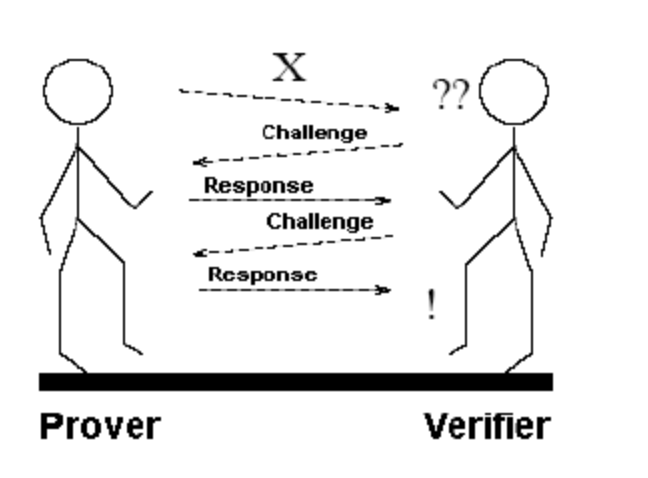
\includegraphics[scale=.5]{Figures/Screen Shot 2023-04-27 at 2.36.17 PM.png}
\end{figure}

We note that being able to compute some arbitrary input can be seen as knowledge. 

Interactive proofs have the verifier prove knowledge of an algorithm by constructing a random sequence of inputs to the algorithm.  \\

\textbf{Example:} A prover wins \(\$1\) for every query successfully completed, and loses \(\$1\) for every query that did not complete successfully. Randomness of inputs makes this a unprofitable high-variance strategy.  \\ 

\textbf{Knowledge Soundness:} If a prover can generate a valid proof then there is a way of reverse engineering their details (algorithm). \\ 

\subsection{Connections to LLMs}

\begin{itemize}
    \item Can a LLM achieve knowledge soundness?
    \item Can we make a prover and verifier LLM interact with each other?
    \item Do LLMs have "knowledge"?
\end{itemize}

Current capacity of langauge models are tested by their success on certain collection of tasks. such as the the Big-Bench Suite, which tests LLMs on over 200 tasks. Recent work found that breaking down these prompts into smaller tasks can drastically improve success (Chain-Of-Thought). \\ 

Let us next very informally define the steps of a LLM: 

\begin{itemize}
    \item Use randomness to initialize model parameters
    \item Text is fed through and the ability to predict certain snippets is checked. 
    \item Humans or automated query generation checks the correctness of these outcomes
\end{itemize}

Mathematically a LLM learns a function \(f(x,r)\) where \(x\) is some text query and \(r\) is some randomness from \(R\) that is used to initiate and maintain training. Consider a query \(x\), if we look at the volume of that set: 
\[
    S = \{(x,r f(,x,r)), r \in R \}
\]     
What does it mean for \(S\) to be large or small? If \(S\) is small no matter \(r\) we end up with similar answers. If \(S\) is large we probably can't  view the answer \(f(x,r)\) as generated by \(x,r\). In other words we gain no knowledge about the data generating process if \(S\) is large. 

Suppose we have some function that maps volume to a scalar value called \(vol(\cdot)\). If \(vol(S)\) is small we have effectively sampled the space of random conclusions different to every weight. Basically a probabilistic form of knowledge soundness. Some researcher believe that \(vol(S)\) is still large, implying that many of this auto-regressive LLMs are not fixable.  \\ 

Let us now consider the idea of breaking up a prompt into many smaller tasks. If such a process was better, this would be saying that \((x_0, r), \ldots (x_l, r) \) is better than \(x_0 \mid x_1 \mid \ldots \mid x_l, r\). This could be thought as a ``anti-fiat-shamir" as the sequential form reintroduces some randomness that is context dependent. We see that knowledge of the process producing the context DOES have an effect unlike what we expect in traditional interactive proofs. 

\subsection{LLM vs LLM}

\textbf{Can LLMs achieve knowledge soundness?}

Assume we have two LLM models, where one was fine-tuned with some warm-up queries \(q_1, \ldots q_n\) and one was a stock LLM. Suppose that the stock LLM is unable to solve a logical query prompted to both LLMs but the fined-tuned LLM was, no matter the chain-of-thought structure of input given to the stock LLM. Let us now consider we have the same two LLMs and we give each a set of \(l\) warm up queries, before asking each a random subset of \(I \in [k]\)  logical queries. If the provided transcript of responses between the LLM converge (halts in polynomial time with respect to \(k, l\) ), then we can modify this approach where we have now the fine tuned model prove to the stock model that is has knowledge the stock does not. The Length of such proof can be used as a heuristic for the knowledge of the fined-tuned model. As such we have a way to construct knowledge between two LLMs and show that a LLM has knowledge. 

\end{document}
